\chapter{Internet of Things}

The main topics addressed aside from \textbf{IoT} itself are how it relates to \textit{Machine Learning} and \textit{Cloud} computing processes, but also \textit{IoT interoperability}, known \textit{Standards}, and the \textit{security} concerns about IoT.

\section{IoT introduction}
\textbf{Cyber and Physical Systems} (CPS) operate in both the Physical and Cyber worlds, thus we can see IoT as an embodiement of CPSs.

In a \textit{smart environment}, smart objects are both physical and cyber, hence they are subject to ``physical experiences'' such as being placed, moved, damaged and so on.
\begin{center}
   But actually\dots\\
   \ul{What is a \textit{smart environment}?}
\end{center}

The answer actually ain't trivial.

\section{Platforms for IoT}
Sensors and actuators are the edge of the cloud.
In general the purpose of IoT is to gather and send data, send it somewhere where it gets transformed into information ultimately used to provide some functionality for an end user, or it simply presented to them.

A \textbf{Platform for IoT} is essentially a ---complex--- software hosted on the cloud, which, first of all, \ul{\textbf{collects} data gathered by IoT devices, but \textit{not} only that}:
\begin{itemize}
   \item Identification
   \item Discovery
   \item Device Management
   \item Abstraction/virtualization
   \item Service composition\\
   Integrating services of different IoT devices and SW components into a composite service
   \item Semantics
   \item Data Flow management
   \begin{itemize}
      \item $sensors \longrightarrow applications$
      \item $applications \ra sensors$
      \item Support for aggregation, processing, analytics
   \end{itemize}
\end{itemize}

\section{No-SQL Databases}
\textbf{No-SQL} DBs address the problem of the several changes of data formats, sources, cardinality and so on, which happen throughout time.

A common example is \textbf{MongoDB}, which stores records in JSON-like objects called \textit{documents}, which are stored in \textit{collections}, the entity corresponding to tables in relational DBs,
with the key difference that multiple documents in a single collection may be structured differently.

\section{IoT Issues}
\begin{paracol}{2}
   
   \begin{itemize}
      \item Performance
   \item Energy Efficiency
   \item Security
   \item Data analysis/processing
   \begin{itemize}
      \item Adaptability/personalization
   \end{itemize}
   \note{The course will cover the basics of signal processing, with mentions to machine learning}
\end{itemize}
\switchcolumn

\begin{itemize}
   \item Communication/brokerage/binding
   \item Data representation
   \item Interoperability
   \note{
      Standard discussed will be ZigBee, MQTT, and IEEE 802.15.4 (?)
      }
   \end{itemize}
\end{paracol}

\begin{figure}[htbp]
   \centering
   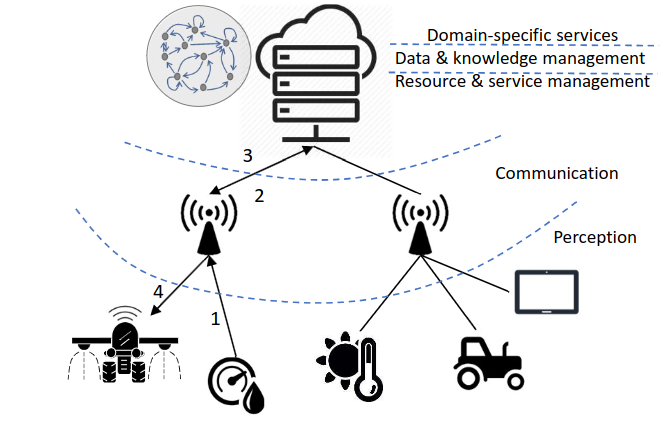
\includegraphics{images/iot_communication.png}
   \caption{Communication outline in IoT}
   IoT systems are distributed, and servers may be dislocated around the globe, making room for \ul{\textbf{latency} and \textbf{reliability} issues}.
   \label{fig:iot_communication}
\end{figure}

To confine the problem displayed in Fig. \ref{fig:iot_communication} there are proposal to move the ability to make a decision on the data closer to the edge, but this in general isn't trivial.

\labelitemize{\textit{\ul{Key Issues}}}{
   \begin{enumerate}
      \item Producing and handling fast-streaming heterogeneous sensed data
      \item Make devices context-aware \& allow them for continuous adaptation
      \item Handle strong computing and energy constraints
   \end{enumerate}
   }

\subsection{Edge and Fog computing}
   \begin{figure}[htbp]
      \centering
      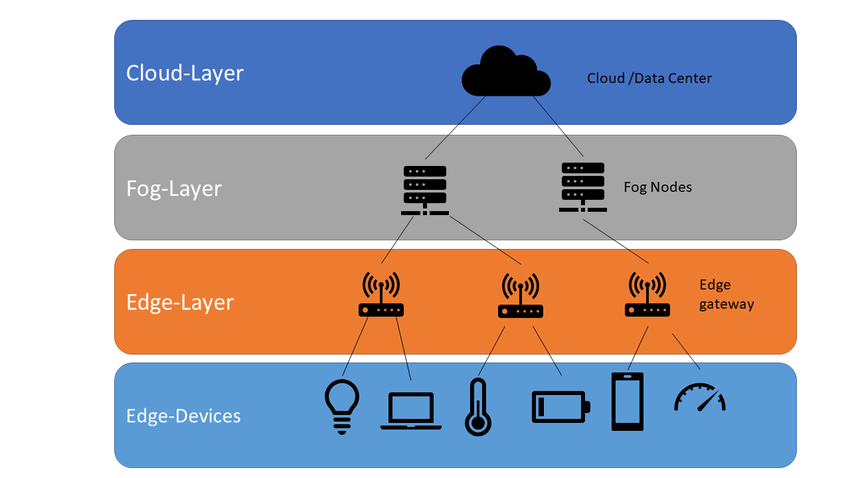
\includegraphics{images/fogedge.png}
      \caption{Layers scheme}
      \label{fig:fogedge}
   \end{figure}
A solution forsees to split the network in 4 layers, allowing for different response times and decisional capabilities.

A gateway on the \textbf{edge} interconnects the IoT-enabled devices with the higher-level communication networks, performing protocol translations.

A basic task performed at the fog layer is  aggregating and collecting data, and then flushing it to the cloud periodically.

However, some decisions on the aggregated data may be taken at the fog node without querying the cloud, for instance determining where is a nest of tortoises, whether an explosion has occurred (by analyzing data from multiple sensors), and ---maybe, one day in a not-so-far future--- recognize human language.
\note{prof. Chessa developed an 8 bit controller implementing a model for determining where is a nest of tortoises.\\
\textit{Alexa} and \textit{Google Home} currently send audio samples to the cloud for processing, but in the futurue this may be done locally.}


\subsection{Artificial Intelligence}
AI splits into \textbf{Machine Learning} and \textbf{Curated Knowledge}.
\note{\textit{ML} focuses on mimicking how humans \ul{\textit{learn}} on new knowledge, while \textit{curated knowledge} focuses on mimicking how humans \ul{\textit{reason}} on a known set of data.}

Machine Learning reveals itself to be particularly useful in aggregatin multiple heterogeneous time-series sensed data about the same environment.
\note{Supervised and Reinforcement learning are more promising than}


\subsection{Blockchain \& IoT}
A \textbf{blockchain} may act as a shared ledger between companies in a supply chain, with IoT devices to track goods and to monitor their quality along the chain, i.e. production stages, shipping and distribution.\\
With a blockchain each actor along the supply chain can \ul{query the ledger to check the ---certified--- state of the goods}.

\subsection{Interoperability}
\labelitemize{\textit{Vertical Silos}}{
   Developing a straight implementation of an IoT solution, starting from physical up to the application layer, is not a problem by itself.\\
   In this way solution you implemented will work only on your devices, making your intervention needed for any change or update;
   besides, products by other vendors will be incompatible. 
}
\textit{Vertical Silos} business model leads to \textbf{vendor lock-in}s, which basically are service limitations which prevent the users from purchasing and using products from other vendors.
\nl
\nl

The solution to avoid ---or limit--- such issues is to introduce \textbf{standards}.

For what concerns wireless communication, standards are mainly differentiated by \textit{Range} and \textit{Data Rate}.


